\section{Iteration 3 -- Math Questions}
\subsection{Q1: Four terms, three documents and a complete SVD}
Use terms $(\text{天},\text{气},\text{足},\text{球})$ and documents
$\text{天气}$, $\text{天气足球}$, $\text{足球}$ in that order.
These are designed toy strings, not news observations.
Counting each term gives
\[
C=\begin{bmatrix}1&1&0\\1&1&0\\0&1&1\\0&1&1\end{bmatrix},
\quad df=(2,2,2,2)^\top,\quad
\alpha=\log(3/2),\quad A=\alpha C\in\R^{4\times3}.
\]
Each row occurs in two of three documents, so the common IDF is $\alpha$ by
the definition of IDF. Matrix multiplication gives
\[
G=A^\top A=\alpha^2 B,\qquad
B=\begin{bmatrix}2&2&0\\2&4&2\\0&2&2\end{bmatrix}.
\]
Expanding the determinant along the first row,
\[
\det(xI-B)=(x-2)\big((x-4)(x-2)-4\big)-4(x-2)
=x(x-2)(x-6).
\]
Thus the eigenvalues of $G$ are $6\alpha^2,2\alpha^2,0$ by scalar
multiplication of eigenvalues. Solving each homogeneous system and
normalizing by the Euclidean norm gives
\[
v_1=\frac{(1,2,1)^\top}{\sqrt6},\quad
v_2=\frac{(1,0,-1)^\top}{\sqrt2},\quad
v_0=\frac{(1,-1,1)^\top}{\sqrt3}.
\]
Their pairwise dot products vanish. The positive singular values are
$\sigma_1=\sqrt6\,\alpha$ and $\sigma_2=\sqrt2\,\alpha$ by taking positive
square roots. Using the Iteration 2 construction $u_i=Av_i/\sigma_i$ gives
\[
u_1=\tfrac12(1,1,1,1)^\top,\qquad
u_2=\tfrac12(1,1,-1,-1)^\top.
\]
These are unit and orthogonal. With $U=[u_1,u_2]$, $V=[v_1,v_2]$,
$\Sigma=\mathrm{diag}(\sigma_1,\sigma_2)$, substitution gives
$U\Sigma V^\top=A$. This is the compact rank-2 SVD; the null vector
does not supply a positive singular direction.

Rank one gives
\[
A_1=u_1\sigma_1v_1^\top
=\frac{\alpha}{2}\begin{bmatrix}1&2&1\\1&2&1\\1&2&1\\1&2&1\end{bmatrix},
\qquad D_1=\alpha(1,2,1)^\top.
\]
Every reduced document is a positive scalar in $\R^1$, so every defined
cosine is one. Originally, the first and third documents are orthogonal;
the other two distinct-document cosines are $1/\sqrt2$, by the dot-product
formula. Rank one retains $6/(6+2)=3/4$ of the energy and has squared
Frobenius error $2\alpha^2$ by the discarded-energy identity.
\input{\resultspath/tiny_cosines.tex}
This example exposes loss of distinction, even though the approximation is
optimal for its rank in Frobenius norm.

\textbf{Independent check.} \path{small_example.py} computes $C^\top C$
with \texttt{Fraction}, evaluates $Gv_i-\sigma_i^2v_i$ and $Gv_0$,
checks $U^\top U=V^\top V=I$, substitutes the factors back into $A$,
and compares the error with $2\alpha^2$. It also runs the shared power
solver and the library checks. Counts and rational products are exact;
logarithms and square roots are stated symbolically and evaluated in
floating point. Appendix A prints the numerical matrices; Appendix B
lists every power iterate. The script prints all stages, including
the starting vectors and convergence diagnostics.

\subsection{Q2: From-scratch functions and their equations}
The shared numerical core is \texttt{src/methods.py}. Every function below
has an equation comment, and the same functions run the tiny example,
the simulation and the real corpus. NumPy's decomposition solvers and
scikit-learn are used only in verification helpers.

\textbf{Steps 1--2: counts and weighting.}
\begin{align}
C_{tj}&=\sum_{x\text{ in document }j}\mathbf1\{x=t\},
&& C\in\R^{m\times n}. \tag{E1}\\
df_t&=\sum_j\mathbf1\{C_{tj}>0\},\quad
w_t=\log(n/df_t),\quad A_{tj}=C_{tj}w_t. \tag{E2}\\
q_t&=C^{\mathrm{query}}_t w_t,
&&q\in\R^m. \tag{E3}
\end{align}
These are \path{my_count_matrix}, \path{my_tfidf} and
\path{my_query_vector}. An unobserved fixed-vocabulary row gets weight
zero without evaluating $\log0$. Queries reuse the fitted vocabulary/IDF.

\textbf{Steps 3--5: Gram matrix, power iteration and deflation.}
\begin{align}
G&=\begin{cases}A^\top A&n\le m\\AA^\top&m<n,\end{cases}
&&G\in\R^{p\times p}. \tag{E4}\\
P_i x&=(I-Q_iQ_i^\top)x,
&&Q_i\in\R^{p\times i}. \tag{E5}\\
x_{\ell+1}&=\frac{P_iG_i x_\ell}{\|P_iG_i x_\ell\|_2},\quad
\lambda=x_{\ell+1}^\top Gx_{\ell+1}. \tag{E6}\\
G_{i+1}&=G_i-\lambda vv^\top,\quad G_0=G. \tag{E7}\\
\sigma_i&=\sqrt{\lambda_i},\qquad
u_i=Av_i/\sigma_i\ \text{(right Gram)},\quad
v_i=A^\top u_i/\sigma_i\ \text{(left Gram)}. \tag{E8}
\end{align}
These correspond to \path{my_gram}, \path{my_reorthogonalize},
\path{my_power_iteration}, \path{my_deflate} and
\path{my_svd_power}. Two passes of (E5) reduce loss of orthogonality.
The smaller left Gram is used for the 50-term simulations when $n>50$;
the right Gram is used for the toy and real matrices.
Both routes are justified by the Iteration 2 SVD-construction proof.

To see why power iteration finds a leading direction, expand
$x_0=\sum_j c_jv_j$ in an orthonormal eigenbasis. Then
$G^\ell x_0=\lambda_1^\ell(c_1v_1+
\sum_{j>1}c_j(\lambda_j/\lambda_1)^\ell v_j)$ by the eigenvector equation.
If $c_1\ne0$ and $\lambda_1>\lambda_2$, normalization suppresses the
other components at a rate controlled by $\lambda_2/\lambda_1$.
For $A^\top A$ this is $(\sigma_2/\sigma_1)^2$.
Deflation works because
$(G-\lambda_1v_1v_1^\top)v_1=0$ and, for $j>1$,
$(G-\lambda_1v_1v_1^\top)v_j=\lambda_jv_j$ by orthogonality.
Repeated values identify a subspace rather than a unique vector.

The fixed starting RNG has seed 0. The stopping test is a projected
deflated-Gram eigen-residual at most $10^{-14}\|G\|_F$, with a maximum
of 200,000 iterations per direction. The original-Gram residual is
also recorded. Eigenvalues at or below $10^{-12}$ of the leading
value are rejected as unresolved, consistent with the earlier cutoff.
Failure to converge or to resolve a positive value raises an error.
Gram construction squares the nonzero condition number and therefore
requires this numerical caution.

\textbf{Steps 6--8: coordinates, similarities, energy and ordering.}
\begin{align}
D&=V_k\Sigma_k\in\R^{n\times k}. \tag{E9}\\
z&=U_k^\top q,\qquad \widehat q=\Sigma_k^{-1}z\in\R^k. \tag{E10}\\
N_i&=X_i/\|X_i\|_2,\qquad S=NN^\top. \tag{E11}\\
s_j&=\frac{D_j^\top z}{\|D_j\|_2\|z\|_2}. \tag{E12}\\
E_k&=\frac{\sum_{i=1}^k\sigma_i^2}{\|A\|_F^2},\qquad
k_*=\min\{k:E_k\ge0.90\}. \tag{E13}\\
\mathrm{matches}&=\text{five largest }s_j\text{ after self-ID exclusion}. \tag{E14}
\end{align}
Ascending ID breaks score ties. These map to
\path{my_document_coordinates}, \path{my_project_query},
\path{my_normalize_rows}, \path{my_cosine_matrix},
\path{my_query_cosines}, \path{my_energy_rank} and
\path{my_top_matches}.

For a document $q=Ae_j$, $U_k^\top q=\Sigma_kV_k^\top e_j$
by orthonormality. Thus the projected query matches row $j$ of $D$,
and the folded query matches row $j$ of $V_k$.
Retrieval compares $z$ with $D$; the fold-in identity compares
$\widehat q$ with $V_k$. Unequal diagonal scaling changes angles.

Counts cost $O(T+mn)$ for $T$ tokens and a dense matrix; TF-IDF costs
$O(mn)$. The smaller Gram costs $O(mnp)$. Direction $i$ costs
$O(t_i(p^2+pi))$ for $t_i$ power steps and reorthogonalization.
Deriving opposite-side factors costs $O(mnk)$. All-pairs cosine costs
$O(n^2k)$ after reduction, compared with $O(n^2m)$ before it.
Working storage is $O(mn+p^2+(m+n)k)$, plus any cosine matrix.

\subsection{Q3: Rank from real-data energy}
The predeclared choice is the smallest rank retaining 90\% of squared
singular-value energy, independently for each tokenization.
This percentage is an analysis choice; the Mandarin handout does not
prescribe one. The identity $\|A\|_F^2=\sum_i\sigma_i^2$
(from orthogonal invariance of the Frobenius norm) supplies the denominator.
The custom solver extracts successive directions until the target is met;
a full NumPy spectrum verifies the result afterward.
\input{\resultspath/real_shapes.tex}
For characters, $E_{\CharRank}=\CharEnergy$ and the previous energy is
\CharPreviousEnergy. For words, $E_{\WordRank}=\WordEnergy$ and the
previous energy is \WordPreviousEnergy. Hence the reported ranks are
minimal for this threshold. The Frobenius tail identity gives
$\|A-A_k\|_F^2/\|A\|_F^2=1-E_k$.
Retaining energy controls squared reconstruction loss, not relevance.
The fairly high ranks reflect lexical variation beyond the few topic labels.
The next/last-retained singular-value ratios are \CharBoundaryRatio{}
and \WordBoundaryRatio{}, so convergence near the cutoff is slower than
for a widely separated leading direction.
\begin{figure}[htbp]\centering
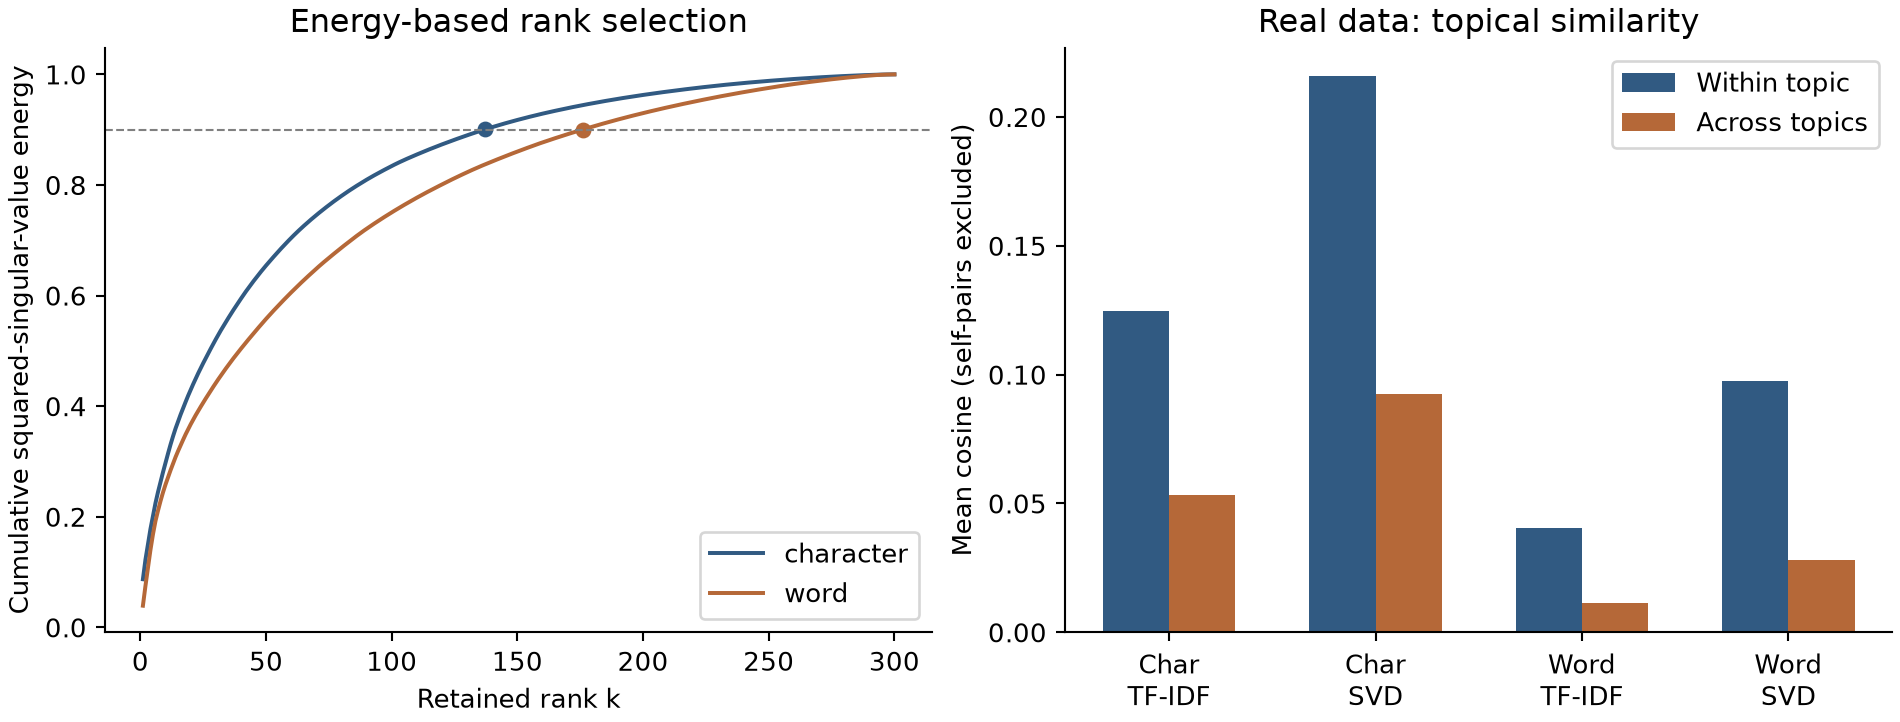
\includegraphics[width=\textwidth]{real_comparison.png}
\caption{Left: full reference energy curves, with custom-selected ranks marked.
Right: measured topic means from the custom representations.}\end{figure}

\subsection{Q4: Characters versus jieba words}
Both representations use exactly the same 300 document IDs and the same
raw-TF/unsmoothed-IDF rule. Character filtering keeps U+4E00--U+9FFF,
as in Iteration 2. Word preprocessing replaces discarded runs by spaces
to preserve boundaries, then uses jieba 0.42.1 precise mode,
\path{cut_all=False}, \texttt{HMM=True}, and its default dictionary.
Only fully Chinese tokens are retained. No stopword list or minimum
frequency is added. The word vocabulary is larger and its matrix is sparser.
\input{\resultspath/real_similarity.tex}
Within/across topic means both rise after SVD, while their difference
also rises. Character nearest-topic agreement is unchanged; word
nearest-topic agreement falls after reduction.
The original word representation has the strongest nearest-topic
agreement among these four settings, despite smaller raw cosines.
Absolute cosines are not directly comparable across different feature
spaces. Each representation has its own energy-selected rank, so the
comparison combines tokenization with the rank implied by the common rule.
Topic labels are a useful proxy, not a judgment of semantic equivalence.

\subsection{Q5: One fixed query and its top five matches}
The query is the full title/body of the first document in the unchanged
sample manifest, \texttt{sports:2}, titled
“冠军球队迎新欢乐派对 黄旭获大奖张军赢下PK赛”.
It describes a golf-party event involving champion athletes.
The choice was fixed before inspecting rankings. Its own ID is excluded.
This is descriptive in-corpus retrieval, with no held-out evaluation.
\input{\resultspath/query_character_original.tex}
\input{\resultspath/query_character_reduced.tex}
The original character ranking puts an education interview first.
The largest positive dot-product terms include individual name characters
such as 煊, 张 and 伟 (recorded in \path{query_term_contributions.csv}).
Such overlaps can connect unrelated names and contexts.
After reduction, \texttt{sports:374} moves from fourth to first, but it
is a basketball report rather than the same golf event.
Some education results remain. The change in angles is real;
the ranking does not establish improved semantic relevance.
\input{\resultspath/query_word_original.tex}
\input{\resultspath/query_word_reduced.tex}
Original word matches include sports reports sharing terms such as
冠军 and 球队. The reduced word ranking contains no sports-labeled
document in its top five. Its first result concerns an event for returning
overseas scholars. Shared broad event language can coexist with a wrong
topic, and projection spreads term weights through the retained subspace.
Terms highlighted from a reconstructed vector need not occur literally
in that article. These results illustrate why energy preservation and
numerical correctness do not guarantee a useful query ranking.
No query or rank was changed to hide this failure case.
